\documentclass[12pt,oneside]{article}
\usepackage[russian,english]{babel}
\usepackage[utf8]{inputenc}
\usepackage{abstract}
\usepackage{amsmath,amssymb,mathrsfs,mathtext,amsthm}
\usepackage{a4wide}
\usepackage[T2A]{fontenc}
\usepackage{subfig}
\usepackage{url}
\usepackage[usenames]{color}
\usepackage{colortbl}

\newcommand{\hdir}{.}
\usepackage{hyperref}       % clickable links
\usepackage{lineno}
\usepackage{graphicx,multicol}
\usepackage{epstopdf}
\usepackage{cite}
\usepackage{amsmath,amssymb,mathrsfs,mathtext}
\usepackage{tikz}
\usetikzlibrary{shapes,arrows,shadows}

\newtheorem{theorem}{Theorem}
\newtheorem{proposition}{Proposition}

\theoremstyle{definition}
\newtheorem{definition}{Definition}

\usepackage{algorithm}
\usepackage[noend]{algcompatible}

\usepackage{multirow}

\usepackage{caption}
\usepackage{geometry}
\usepackage{setspace}
%\onehalfspacing
\renewcommand{\baselinestretch}{1.5}
\geometry{verbose,a4paper,tmargin=2cm,bmargin=2cm,lmargin=3cm,rmargin=1.5cm}

\usepackage[center]{titlesec}
\renewcommand{\refname}{REFERENCES}
% \renewcommand{\contentsname}{REFERENCES}
\titlelabel{\thetitle.\quad}
\newcommand{\sectionbreak}{\clearpage}
\let\originalparagraph\paragraph
\renewcommand{\paragraph}[2][.]{\originalparagraph{#2#1}}
\titleformat{\section}[block]{\Large\bfseries\filcenter}{\thesection.\;}{0.1em}{\uppercase}

\titleformat{\subsection}[block]{\large\bfseries\filcenter}{\thesubsection.\;}{0.1em}{}
\titleformat{\subsubsection}[block]{\bfseries\filcenter}{\thesubsubsection.\;}{0.1em}{} 

\newcommand{\bx}{\mathbf{x}}
\newcommand{\by}{\mathbf{y}}
\newcommand{\bw}{\mathbf{w}}
\newcommand{\ba}{\mathbf{a}}
\newcommand{\bz}{\mathbf{z}}
\newcommand{\bb}{\mathbf{b}}
\newcommand{\bY}{\mathbf{Y}}
\newcommand{\bX}{\mathbf{X}}
\newcommand{\bu}{\mathbf{u}}
\newcommand{\bt}{\mathbf{t}}
\newcommand{\bp}{\mathbf{p}}
\newcommand{\bq}{\mathbf{q}}
\newcommand{\bc}{\mathbf{c}}
\newcommand{\bP}{\mathbf{P}}
\newcommand{\bT}{\mathbf{T}}
\newcommand{\bB}{\mathbf{B}}
\newcommand{\bQ}{\mathbf{Q}}
\newcommand{\bC}{\mathbf{C}}
\newcommand{\bE}{\mathbf{E}}
\newcommand{\bF}{\mathbf{F}}
\newcommand{\bU}{\mathbf{U}}
\newcommand{\bW}{\mathbf{W}}
\newcommand{\bbR}{\mathbb{R}}
\newcommand{\cA}{\mathcal{A}}
\newcommand{\T}{\mathsf{T}}
\newcommand{\bchi}{\boldsymbol{\chi}}
\newcommand{\bnu}{\boldsymbol{\nu}}
\newcommand{\bmu}{\boldsymbol{\mu}}
\newcommand{\btheta}{\boldsymbol{\theta}}
\newcommand{\bTheta}{\boldsymbol{\Theta}}
\newcommand{\bOne}{\boldsymbol{1}}
\newcommand{\bZero}{\boldsymbol{0}}
\newcommand{\argmin}{\mathop{\arg \min}\limits}
\newcommand{\argmax}{\mathop{\arg \max}\limits}

\newcommand\undermat[2]{%
	\makebox[0pt][l]{$\smash{\underbrace{\phantom{%
					\begin{matrix}#2\end{matrix}}}_{\text{$#1$}}}$}#2}

\begin{document}

\setcounter{page}{3}
\begin{center}
	Dimensionality reduction for multivariate signal decoding problem\\ 
	Roman Isachenko \\[5mm]
	Submitted to the Skolkovo Institute of Science and Technology 
	on 01 June 2018 \\[5mm]
	\textbf{ABSTRACT:} 
\end{center}

This study is devoted to the problem of signal decoding for Brain Computer Interface~(BCI) modelling. 
BCI helps disabled people to recover their mobility.
The goal of the research is to build a model which predicts a limb position by brain signals. 
The challenge of the investigation is redundancy in data description. 
High correlation in measurements leads to correlation in input space. 
Additionally, the target space are correlated due to dependent consequent hand positions.

To overcome correlations in feature representation, feature selection are used.
However, the majority of feature selection methods ignore the dependencies in the target space.
We suggest a novel approach to feature selection in multivariate regression.
To take into account the correlations in the target matrix, the proposed approach extend the ideas of the quadratic programming feature selection~(QPFS) algorithm. 
The QPFS algorithm select non-correlated features, which are relevant to the targets. The proposed methods weigh the targets by their importances.

The computational experiment was carried out on the real public electrocorticogram (ECOG) dataset. 
The proposed algorithms show high performance compared to the known strategy.
We analyze the robustness of the predictive model and the stability of the selected feature sets.\\[5mm]
Skoltech Research Advisor: \\
Name: Maxim Fedorov \\
Degree: {\color{red} TO DO} \\
Title: {\color{red} TO DO} \\[5mm]
MIPT Research Advisor: \\
Name: Vadim Strijov \\
Degree:{\color{red} TO DO} \\
Title: {\color{red} TO DO}

\newpage
\tableofcontents

\newpage
%%%%%%%%%%%%%%%%%%%%%%%%%%%%%%%%%%%%%%%%%%%%%%%%
\section{Introduction}
%%%%%%%%%%%%%%%%%%%%%%%%%%%%%%%%%%%%%%%%%%%%%%%%
The research investigates the problem of signal decoding for Brain Computer Interface (BCI)~\cite{costecalde2018long}. 
BCI aims to develop systems that help people with a severe motor control disability to recover mobility.
The minimally-invasive implant records cortical signals and the model decodes them on real time to predict the coordinates of an exoskeleton limbs~\cite{mestais2015wimagine,eliseyev2014clinatec}.
The subject placed inside the exoskeleton can drive it by imagining movements as if they were making the movement by themselves. 

The challenge to build such model is redundancy in initial data description. 
The features are highly multicorrelated due to spatial nature of the data. 
The brain sensors are close to each other. 
It leads to the redundant measurements and instability of the final model.
In addition, the redundant data description requires excess computations which lead to real-time delay. 
To overcome this problem dimensionality reduction~\cite{chun2010sparse,mehmood2012review} or feature selection~\cite{katrutsa2015stress,li2017feature} methods are used.

The dimensionality reduction algorithms find the optimal combinations of the initial features and use these combinations as the model features. 
For ECoG-based data the most suitable dimensionality reduction algorithm is partial least squares~(PLS)~\cite{eliseyev2014stable,engel2017kernel,eliseyev2012l1}. 
The algorithm projects the features and the targets onto the joint latent space and maximizes the covariances between projected vectors. 
It allows to save information about initial input and target matrices and find their relations. 
The dimensionality of latent space is much less than the size of initial data description. It leads to stable linear model built at the small number of features. 
The overview of recent advances in PLS algorihms is given in~\cite{rosipal2006overview,rosipal2011nonlinear}.
In this case we obtain the linear model with small latent dimension.
However, the final model use the whole range of the initial features and it does not allow to detect useless features. 

Feature selection is a special case of dimensionality reduction when the latent representation is choosen as a subset of initial data description. 
Here the model are built on the subset of the features. 
One of the approach to feature selection is to maximize feature relevances and minimize pairwise feature redundancy. 
This approach was recently proposed and investigated in~\cite{ding2005minimum,yamada2014high}.
Quadratic programmic feature selection~(QPFS)~\cite{rodriguez2010quadratic} uses this approach to construct the optimization problem. It was shown in~\cite{katrutsa2017comprehensive} that QPFS algorithm outperforms many existing feature selection methods for the univariate regression problem. 
The QPFS algorithm introduces two functions: $\text{Sim}$ and $\text{Rel}$.
$\text{Sim}$ estimates the redundancy between features, $\text{Rel}$ contains relevances between each feature and the target vector.
QPFS minimizes the function Sim and maximizes the function Rel simultaneously.
The algorithm solves the following optimization problem
\begin{equation}
(1 - \alpha) \cdot \underbrace{\bz^{\T} \bQ \bz}_{\text{Sim}(\bX)} - \alpha \cdot \underbrace{\vphantom{()} \bb^{\T} \bz}_{\text{Rel} (\bX, \bnu)} \rightarrow \min_{\substack{\bz \geq \bZero_n \\ \bOne_n^{\T} \bz=1}}.
\label{eq:qpfs_problem}
\end{equation}
The matrix $\bQ \in \bbR^{n \times n}$ entries measure the pairwise similarities between features.
The vector $\bb \in \bbR^n$ expresses the similarities between each feature and the target vector.
The normalized vector~$\bz$ shows the importance of each feature.
The function~\eqref{eq:qpfs_problem} penalizes the dependent features by the function Sim and encourages features relevant to the target by the function Rel.
The parameter~$\alpha$ controls the trade-off between Sim and the Rel.
To measure similarity the authors use the absolute value of sample correlation coefficient or sample mutual information coefficient between pairs of features for the function Sim, and between the features and the target vector for the function Rel.

The paper~[{\color{red} MOTRENKO}] proposes a multi-way version of QPFS algorithm for tensor ECoG-based data. 
It was shown that QPFS is appropriate feature selection method for brain signal decoding problem.
We consider the multivariate problem, where the dependent variable is a vector. 
It refers to the prediction of limb position for not just one timestamp, but for some period of time. 
The subsequent hand positions are correlated. 
It leads to correlations in the model targets. 
In this situation feature selection algorithms do not take into account these dependencies.
Hence, the selected feature subset is not optimal.
We propose methods to take into account the dependencies in both input and output spaces. 
It allows to get the stable model with fewer variables.
We refer to the original QPFS algortihm as our baseline for the computational experiment.

The experiment was carried out in the ECoG data from the NeuroTycho project~\footnote{\href{http://neurotycho.org/food-tracking-task}{http://neurotycho.org/food-tracking-task}}. 
We compared the proposed methods for multivariate feature selection with the baseline strategy and with PLS algporithm. 
The stability of the proposed methods were investigated.
The proposed algorithms outperform the baseline algorithm and select the less number number of the features. [{\color{red} EXTEND}].

\newpage
%%%%%%%%%%%%%%%%%%%%%%%%%%%%%%%%%%%%%%%%%%%%%%%%
\section{Problem statement}
%%%%%%%%%%%%%%%%%%%%%%%%%%%%%%%%%%%%%%%%%%%%%%%%
\subsection{Multivariate regression}
The goal is to forecast a dependent variable $\by \in \bbR^r$ with $r$ targets from an independent input object $\bx \in \bbR^n$ with $n$ features.
We assume there is a linear dependence
\begin{equation}
	\by = \bTheta \bx+ \boldsymbol{\varepsilon}
	\label{eq:model}
\end{equation}
between the object $\bx$ and the target variable $\by$,
where $\bTheta \in \bbR^{r \times n}$ is a matrix of model parameters, $\boldsymbol{\varepsilon} \in \bbR^{r}$ is a residual vector.
One has to find the matrix of the model parameters~$\bTheta$ given a dataset $\left( \bX, \bY \right)$, where $\bX \in \bbR^{m \times n}$ is a design matrix, $\bY \in \bbR^{m \times r}$ is a target matrix
\begin{equation}
	\bX = [\bx_1, \dots, \bx_m]^{\T} =  [\bchi_1, \dots, \bchi_n]; \quad \bY = [\by_1, \dots, \by_m]^{\T} =  [\bnu_1, \dots, \bnu_r].
\end{equation}
The columns~$\bchi_j$ of the matrix~$\bX$ respond to object features.

The optimal parameters are determined by minimization of an error function.
Define the quadratic loss function:
\begin{equation}
	\mathcal{L}(\bTheta | \bX, \bY) = {\left\| \underset{m \times r}{\mathbf{Y}}  - \underset{m \times n}{\bX} \cdot \underset{r \times n}{\bTheta}^{\T} \right\| }_2^2 \rightarrow\min_{\bTheta}.
\label{eq:loss_function}
\end{equation}
The solution of~\eqref{eq:loss_function} is given by
 \begin{equation}
 	\bTheta = \bY^{\T} \bX (\bX^{\T} \bX)^{-1}.
 \end{equation}

 The linear dependent columns of the matrix $\bX$ leads to an instable solution for the optimization problem~\eqref{eq:loss_function}.
 If there is a vector $\boldsymbol{\alpha} \neq \bZero_n$ such that $\bX \boldsymbol{\alpha}= \bZero_m$, then adding the vector~$\boldsymbol{\alpha}$ to any column of the matrix~$\bTheta$ does not change the value of the loss function $\mathcal{L}(\bTheta | \bX, \bY)$.
 In this case the matrix~$\bX^{\T} \bX$ is not invertible.
 To avoid the strong linear dependence, dimensionality reduction and feature selection techniques are used.
 
 
 %%%%%%%%%%%%%%%%%%%%%%%%%%%%%%%%%%%%%%%%%%%%%%%%
 \subsection{Dimensionality reduction}
 %%%%%%%%%%%%%%%%%%%%%%%%%%%%%%%%%%%%%%%%%%%%%%%%

To eliminate the linear dependence and reduce the dimensionality of the input space, the principal components analysis (PCA) is widely used algorithm. 
The main disadvantage of the PCA method is its insensitivity to the interrelation between the features and the targets.
The partial least squares algorithm projects the design matrix~$\bX$ and the target matrix~$\bY$ to the latent space with low dimensionality ($l < r < n$).
The PLS algorithm finds the latent space matrices $\bT, \bU \in \mathbb{R}^{m \times l}$ that best describe the original matrices~$\bX$ and~$\bY$.

The design matrix~$\bX$ and the target matrix~$\bY$ are projected into the latent space in the following way:
\begin{align}
\label{eq:PLS_X}
\underset{m \times n}{\vphantom{\bQ}\bX} 
&= \underset{m \times l}{\vphantom{\bQ}\bT} \cdot \underset{l \times n}{\vphantom{\bQ}\bP^{\T}} + \underset{m \times n}{\vphantom{\bQ}\bF} 
= \sum_{k=1}^l \underset{m \times 1}{\vphantom{\bp_k^{\T}}\bt_k} \cdot \underset{1 \times n}{\bp_k^{\T}} + \underset{m \times n}{\vphantom{\bp_k^{\T}}\bF},\\
\label{eq:PLS_Y}
\underset{m \times r}{\vphantom{\bQ}\bY} 
&= \underset{m \times l}{\vphantom{\bQ}\bU} \cdot \underset{l \times r}{\bQ^{\T}} + \underset{m \times r}{\vphantom{\bQ}\bE}
=  \sum_{k=1}^l  \underset{m \times 1}{\vphantom{\bq_k^{\T}}\bu_k} \cdot \underset{1 \times r}{\bq_k^{\T}} +  \underset{m \times r}{\vphantom{\bq_k^{\T}}\bE},
\end{align}
where $\bT$ and $\bU$ are scores matrices in the latent space; $\bP$ and $\bQ$ are loading matrices; $\bE,\ \bF$ are residual matrices. PLS maximizes the linear relation between columns of matrices~$\bT$ and~$\bU$
\begin{equation}
\bU \approx \bT \bB, \quad \bB = \text{diag}(\beta_k), \quad \beta_k = \bu_k^{\T}\bt_k / (\bt_k^{\T}\bt_k).
\end{equation}

We use the PLS algorithm as the dimensionality reduction algorithm in this research.
The theoretical explanation of the PLS algorithm are given in section~\ref{sec:pls}.

 %%%%%%%%%%%%%%%%%%%%%%%%%%%%%%%%%%%%%%%%%%%%%%%%
 \subsection{Feature selection}
 %%%%%%%%%%%%%%%%%%%%%%%%%%%%%%%%%%%%%%%%%%%%%%%%
 Feature selection is a special case of dimensionality reduction, where the loading matrices~$\bT$ and $\bU$ are the submtrices of the design matrix $\bX$ and the target matrix~$\bY$.
 
 The feature selection goal is to find the boolean vector~$\ba = \{0, 1\}^n$, which components indicate whether the feature are selected. 
 To obtain the optimal vector~$\ba$ among all possible $2^n - 1$ options, introduce the feature selection error function $S(\ba | \bX, \bY)$. 
 We state the feature selection problem as follows 
\begin{equation}
	\ba = \argmin_{\ba' \in \{0, 1\}^n} S(\ba' | \bX, \bY).
	\label{eq:feature_selection}
\end{equation}
The goal of feature selection is to construct the appropriate function~$S(\ba | \bX, \bY)$. The particular examples for the considered feature selection algorithms are given below and summarizes in the Table~\ref{tbl:summary}.

The problem~\ref{eq:feature_selection} are hard to solve due to discrete binary domain~$\{0, 1\}^n$. We relax the problem~\ref{eq:feature_selection} to the continuous domain~$[0, 1]^n$. The relaxed feature selection problem is
\begin{equation}
\bz = \argmin_{\bz' \in [0, 1]^n} S(\bz' | \bX, \bY).
\label{eq:relaxed_feature_selection}
\end{equation}
Here vector~$\bz$ is a normalized feature scores.
Firstly, solve the problem~\ref{eq:relaxed_feature_selection} to obtain the feature scores~$\bz$. 
Then the solution of~\ref{eq:feature_selection} is recovered by thresholding:
\begin{equation}
\ba = [a_j]_{j=1}^n, \quad 
a_j = \begin{cases}
1, & z_j > \tau; \\
0, & \text{otherwise}.
\end{cases}
\end{equation}
Here the value~$\tau$ is a hyperparameter. 

Once the solution~$\ba$ of~\eqref{eq:feature_selection} is known, the problem~\eqref{eq:loss_function} becomes
\begin{equation}
\mathcal{L}(\bTheta_{\ba} | \bX_{\ba}, \bY) = {\left\| \mathbf{Y} - \bX_{\ba}\bTheta^{\T}_{\ba} \right\| }_2^2 \rightarrow\min_{\bTheta_{\ba}},
\end{equation}
where the subscript~$\ba$ indicates the submatrix with the columns for which components of~$\ba$ equal 1.

\subsection{Quadratic Programming Feature Selection}
Our base algorithm for feature selection is quadratic programming feature selection algorithm. 
The QPFS algorithm selects non-correlated features, which are relevant to the target vector~$\bnu$ for the linear regression problem with~$r=1$
\begin{equation}
	\| \bnu - \bX \btheta\|_2^2 \rightarrow\min_{\btheta \in \bbR^{n}}.
\end{equation}

The authors of the original QPFS paper suggested the way to select~$\alpha$ for~\ref{eq:qpfs_problem} and make $\text{Sim}(\bX)$ and $\text{Rel}(\bX, \bnu)$ impacts the same:
\begin{equation}
	\alpha = \frac{\overline{\bQ}}{\overline{\bQ} + \overline{\bb}},
\end{equation}
where $\overline{\bQ}$, $\overline{\bb}$ are the mean values of~$\bQ$ and $\bb$ respectively. The QPFS parameters are defined as follows:
\begin{equation}
	\bQ = \left[\text{sim}(\bchi_i, \bchi_j)\right]_{i,j=1}^n, \quad \bb = \left[\text{sim}(\bchi_i, \bnu)\right]_{i=1}^n.
	\label{eq:qpfs_1d_qb}
\end{equation}
Here the function~$\text{sim}(\cdot, \cdot)$ is a similarity measure.
The common ways to define this function are the absolute value of sample Pearson correlation coefficient
\begin{equation}
	\text{sim}(\bchi, \bnu) = |\text{corr}(\bchi, \bnu)| = \left|\frac{\sum_{i=1}^m(\bchi_i - \overline{\bchi})( \bnu_i - \overline{\bnu})}{\sqrt{\sum_{i=1}^m(\bchi_i - \overline{\bchi})^2\sum_{i=1}^m(\bnu_i - \overline{\bnu})^2}}\right|,
	\label{eq:corr_coef}
\end{equation}
or the sample mutual information coefficient
\begin{equation}
\text{sim}(\bchi, \bnu) = I(\bchi, \bnu) = \int \int p(\bchi, \bnu) \log(\frac{p(\bchi, \bnu)}{p(\bchi)p(\bnu)}) d\bchi d\bnu,
\end{equation}
We use the correlation coefficient~\eqref{eq:corr_coef} as a similarity measure~$\text{sim}(\cdot, \cdot)$.
The other ways to define $\bQ$ and $\bb$ are considered in~\cite{katrutsa2017comprehensive}.

The problem~\eqref{eq:qpfs_problem} is convex if the matrix~$\bQ$ is positive semidefinite. In general it is not always true.
To satisfy this condition, the matrix~$\bQ$ spectrum is shifted and the matrix~$\bQ$ is replaced by $\bQ - \lambda_{\text{min}} \mathbf{I}$, where $\lambda_{\text{min}} $ is a $\bQ$ minimal eigenvalue.
The original paper~\cite{rodriguez2010quadratic} suggests the way to solve the quadratic problem~\eqref{eq:qpfs_problem} efficiently. In~\cite{prasad2013scaling} the sequential minimal optimization framework is proposed for solving~\eqref{eq:qpfs_problem}.

%%%%%%%%%%%%%%%%%%%%%%%%%%%%%%%%%%%%%%%%%%%%%%%%
\section{Partial least squares regression}
\label{sec:pls}
%%%%%%%%%%%%%%%%%%%%%%%%%%%%%%%%%%%%%%%%%%%%%%%%

The pseudocode of the PLS regression algorithm is given in the algorithm~\ref{PLSR_code}.
In each of the~$l$ steps the algorithm iteratively calculates columns $\bt_k$, $\bu_k$, $\bp_k$, $\bq_k$ of the matrices $\bT$, $\bU$, $\bP$, $\bQ$, respectively. 
After the computation of the next set of vectors, the one-rank approximations are subtracted from the matrices~$\bX$,~$\bY$. 
This step is called a matrix deflation.
In the first step one has to normalize the columns of the original matrices (subtract the mean and divide by the standard deviation).
During the test mode we need to normalize test data, compute the model prediction~\eqref{eq:model}, and then perform the reverse normalization.

\begin{algorithm}[h]
	\caption{PLSR algorithm}
	\label{PLSR_code}
	\begin{algorithmic}[1]
		\REQUIRE $\bX, \bY, l$;
		\ENSURE $\bT, \bP, \bQ$;
		\STATE normalize matrices $\bX$ и $\bY$ by columns
		\STATE initialize $\bu_0$ (the first column of $\bY$)
		\STATE $\bX_1 = \bX; \bY_1 = \bY$
		\FOR{$k=1,\dots, l$}
		\REPEAT
		\vspace{0.1cm}
		\STATE $\bw_k := \bX_k^{\T} \bu_{k-1} / (\bu_{k-1}^{\T} \bu_{k-1}); \quad \bw_k: = \frac{\bw_k}{\| \bw_k \|}$
		\vspace{0.1cm}
		\STATE $\bt_k := \bX_k \bw_k$
		\vspace{0.1cm}
		\STATE $\bc_k := \bY_k^{\T} \bt_k / (\bt_k^{\T} \bt_k); \quad \bc_k: = \frac{\bc_k}{\| \bc_k \|}$
		\vspace{0.1cm}
		\STATE $\bu_k := \bY_k \bc_k$
		\UNTIL{$\bt_k$ stabilizes}
		\vspace{0.1cm}
		\STATE $\bp_k:= \bX_k^{\T}\bt_k/(\bt_k^{\T}\bt_k),\ 
		\bq_k := \bY_k^{\T}\bu_k/(\bu_k^{\T}\bu_k)$
		\vspace{0.2cm}
		\STATE $\bX_{k+1} :=  \bX_k - \bt_k \bp_k^{\T}$
		\vspace{0.2cm}
		\STATE $\bY_{k + 1} :=  \bY_k - \bu_k \bq_k^{\T} \approx  \bY_k - \bt_k \cdot \left(\frac{\bY^{\T}\bt_k}{\bt_k^{\T}\bt_k}\right)^{\T} $ 
		\ENDFOR
	\end{algorithmic}
\end{algorithm}

The vectors $\bt_k$ and $\bu_k$ from the inner loop of the algorithm~\ref{PLSR_code} contain information about the design matrix $\bX$ and the target matrix $\bY$, respectively. 
The blocks of steps (6)--(7) and (8)-(9)~are analogues of the PCA algorithm for the matrices~$\bX$ and~$\bY$~\cite{geladi1986partial}. 
Sequential repetition of the blocks takes into account the interaction between the matrices~$\bX$ and~$\bY$.

The theoretical explanation of the PLS algorithm follows from the statements.
\begin{proposition}
	The best description of the matrices $\bX$ and $\bY$ taking into account their interrelation is achieved by maximization of the covariance between the vectors $\bt_k$ and $\bu_k$.
\end{proposition}
The statement follows from the equation
\begin{equation}
\text{cov} (\bt_k, \bu_k) = \text{corr} (\bt_k, \bu_k) \cdot \sqrt{\text{var}(\bt_k)} \cdot \sqrt{\text{var}(\bu_k)}.
\end{equation}
Maximization of the vectors $\bt_k$ and $\bu_k$ variances corresponds to keeping information about original matrices, the correlation of these vectors corresponds to interrelation between $\bX$ and~$\bY$. $\blacksquare$

In the inner loop of the algorithm~\ref{PLSR_code} the normalized weight vectors $\bw_k$ and $\bc_k$ are calculated. 
These vectors construct the matrices $\bW$ and $\bC$, respectively.

\begin{proposition}
	The vector $\bw_k$ and $\bc_k$ are eigenvectors of the matrices $\bX_k^{\T} \bY_k \bY_k^{\T} \bX_k$ and $\bY_k^{\T} \bX_k \bX_k^{\T} \bY_k$, corresponding to the maximum eigenvalues.
	
	\begin{align}
	\bw_k \varpropto \bX_k^{\T} \bu_{k-1} \varpropto \bX_k^{\T} \bY_k \bc_{k-1} \varpropto \bX_k^{\T} \bY_k \bY_k^{\T} \bt_{k-1} \varpropto \bX_k^{\T} \bY_k \bY_k^{\T} \bX_k \bw_{k-1}, \\
	\bc_k \varpropto \bY_k^{\T} \bt_k \varpropto \bY_k^{\T} \bX_k \bw_k \varpropto \bY_k^{\T} \bX_k \bX_k^{\T} \bu_{k-1} \varpropto \bY_k^{\T} \bX_k \bX_k^{\T} \bY_k \bc_{k-1},
	\end{align}
	where the $\varpropto$ symbol means equality up to a multiplicative constant.
	\label{st:eig}
\end{proposition}

The statement follows from the fact that the update rule for vectors~$\bw_k$,~$\bc_k$ coincides with the iteration of the power method for the maximum eigenvalue.

Let a matrix~$\mathbf{A}$ be diagonalizable, $\bx$~be some vector, then
\begin{equation}
\lim_{k \rightarrow \infty} \mathbf{A}^k \bx = \lambda_{\max}(\mathbf{A}) \cdot \mathbf{v}_{\max},
\end{equation}
where $\mathbf{v}_{\max}$~is the eigenvector~$\mathbf{A}$, corresponding to the maximum eigenvalue~$ \lambda_{\max} (\mathbf{A})$.
$\blacksquare$

\begin{proposition}
	The update rule for the vectors in steps (6)--(9) of the algorithm~\ref{PLSR_code} corresponds to the maximization of the covariance between the vectors $\bt_k$ and $\bu_k$.
\end{proposition}

The maximum covariance between the vectors $\bt_k$ and $\bu_k$ is equal to the maximum eigenvalue of the matrix $\bX_k^{\T} \bY_k \bY_k^{\T} \bX_k$:
\begin{multline}
\max_{\bt_k, \bu_k}  \text{cov} (\bt_k, \bu_k)^2 = \max_{\substack{\|\bw_k\|=1 \\ \|\bc_k\| = 1}} \text{cov} \left( \bX_k \bw_k, \bY_k \bc_k \right)^2 = \max_{\substack{\|\bw_k\|=1 \\ \|\bc_k\| = 1}} \text{cov} \left(\bc_k^{\T}  \bY_k^{\T} \bX_k \bw_k \right)^2 = \\
= \max_{\|\bw_k\| = 1} \text{cov} \left\|\bY_k^{\T} \bX_k \bw_k \right\|^2 = \max_{\|\bw_k\| = 1} \bw_k^{\T} \bX_k^{\T} \bY_k \bY_k^{\T} \bX_k \bw_k = \\
 = \lambda_{\max} \left( \bX_k^{\T} \bY_k \bY_k^{\T} \bX_k \right),
\end{multline}
where $ \lambda_{\max} (\mathbf{A})$~is the maximum eigenvalue of the matrix $\mathbf{A}$.
Using the statement~\ref{st:eig}, we obtain the required result.
$\blacksquare$

After the inner loop the following step (11) is to compute vectors $\bp_k$, $\bq_k$ by projection of the matrices $\bX_k$ and $\bY_k$ columns to the vector $\bt_k$. 
Before proceeding with the next iteration one has to deflate the matrices $\bX_k$ and $\bY_k$ by the one-rank approximations $\bt_k \bp_k^{\T}$ and $\bt_k \bq_k^{\T}$
\begin{align}
\bX_{k + 1} &= \bX_{k} - \bt_k \bp_k^{\T} = \bX - \sum_k \bt_k \bp_k^{\T}, \\
\bY_{k + 1} &= \bY_{k} - \bt_k \bq_k^{\T} = \bY - \sum_k \bt_k \bq_k^{\T}.
\end{align}
Each next vector $\bt_{k+1}$ turns out to be orthogonal to all vectors $\bt_i$, $i=1, \dots, k$.

Let assume that the dimension of the input, the target, and the latent spaces are equal to~2 ($n = r = l = 2$).
Figure~\ref{fig:PLSFigure} shows the result of the PLS algorithm in this case.
Blue and green dots represent the rows of the matrices~$\bX$ and~$\bY$, respectively. 
The dots were generated from a normal distribution with zero expectation. 
Contours of the distribution covariance matrices are shown in red.
Black contours are unit circles. 
Red arrows correspond to principal components for the set of points. 
Black arrows correspond to the vectors of the matrices~$\bW$ and~$\bC$ from the PLS algorithm. 
The vectors~$\bt_k$ and~$\bu_k$ are equal to the projected matrices~$\bX_k$ and~$\bY_k$ to the vectors~$\bw_k$ and~$\bc_k$, respectively, and are denoted by black pluses. 
Taking into account the interaction between the matrices~$\bX$ and~$\bY$ the vectors~$\bw_k$ and~$\bc_k$ deviate from the principal components directions. 
The deviation of the vectors~$\bw_k$ is insignificant. 
In the first iteration, $\bc_1$ is close to the principal component~$\textit{pc}_1$, but the vectors~$\bc_k$ in the next iterations could strongly correlate. 
The difference in the vectors~$\bw_k$ and~$\bc_k$ the behaviour is associated with the deflation process. In particular, we subtract from~$\bY$ the one-rank approximation found in the space of the design matrix~$\bX$.
\begin{figure}[h]
	\centering
	\includegraphics[width=\linewidth]{figs/PLSFigure.eps}
	\caption{The result of the PLS algorithm for the case $n = r = l = 2$}.
	\label{fig:PLSFigure}
\end{figure}

To obtain the model prediction and find the model parameters, multiply the both hand sides of the~\eqref{eq:PLS_X} by the matrix~$\bW$. 
Since the residual matrix~$\bE$ rows are orthogonal to the columns of the matrix~$\bW$, we have
\begin{equation}
\bX \bW = \bT \bP^{\T} \bW.
\end{equation}
The linear transformation between objects in the input and latent spaces has the form
\begin{equation}
\bT = \bX \bW^*, \quad \text{where } \bW^* = \bW (\bP^{\T} \bW)^{-1}.
\label{eq:W*}
\end{equation}
The matrix of the model parameters~\ref{eq:model} could be found from equations~\eqref{eq:PLS_Y},~\eqref{eq:W*}
\begin{equation}
\bY = \bU \bQ^{\T} + \bE \approx \bT \bB \bQ^{\T}+ \bE = \bX \bW^* \bB \bQ^{\T} + \bE = \bX \bTheta + \bE.
\label{eq:pls_model}
\end{equation}
Thus, the model parameters~\eqref{eq:model} are equal to
\begin{equation}
\bTheta = \bW (\bP^{\T} \bW)^{-1} \bB \bQ^{\T}.
\label{eq:model_parameters}
\end{equation}

The final model~\eqref{eq:pls_model} is a linear model which are low-dimensional in the latent space. 
It reduces the data redundancy and improves the model stability. 

\newpage
\section{Multivariate QPFS}

We are aimed to propose the algorithms which suitable for feature selection in multivariate case. 
If the target space is multidimensional it prone to redundancy and correlations between the targets. 
In this section we consider the algorithms that take into account the probable dependencies in both input and target spaces.

\subsection{Relevance aggregation (RelAgg).}

First approach to apply the QPFS algorithm to the multivariate case ($r > 1$) is to aggregate feature relevances through all $r$ components. The term $\text{Sim}(\bX)$ is still the same, the matrix $\bQ$ is defined by~\eqref{eq:qpfs_1d_qb}. The vector $\bb$ is aggregated across all targets and is defined by
\begin{equation}
\bb = \left[\sum_{k=1}^r\left|\text{corr}(\bchi_i, \bnu_k)\right|\right]_{i=1}^n.
\end{equation}

The drawback of this approach is that it does not use the dependencies in the columns of the matrix $\bY$. Observe the following example:
\begin{equation}
	\bX = [\bchi_1, \bchi_2, \bchi_3], \quad \bY = [\underbrace{\bnu_1, \bnu_1, \dots, \bnu_1}_{r-1}, \bnu_2],
\end{equation}
We have three features and $r$ targets, where first $r-1$ target are identical.
The pairwise features similarities are given by the matrix $\bQ$.
The matrix $\bB$ entries show pairwise features relevances to the targets.
The vector $\bb$ is obtained by summation of the matrix $\bB$ over columns.
\begin{equation}
	\bQ = \begin{bmatrix} 1 & 0 & 0\\ 0 & 1 & 0.8 \\ 0 & 0.8 & 1 \end{bmatrix}, \quad
	\bB = \begin{bmatrix} 0.4 & \dots & 0.4 & 0 \\ 0.5 & \dots & 0.5 & 0.8 \\ \undermat{r-1}{0.8 & \dots & 0.8} & 0.1 \end{bmatrix}, \quad
	\bb = \begin{bmatrix} (r-1) \cdot 0.4 + 0 \\ (r-1) \cdot 0.5 + 0.8 \\ (r-1) \cdot 0.8 + 0.1. \end{bmatrix}
	\label{eq:qpfs_example}
\end{equation}
	\vspace{0.5cm} \\
We would like to select only two features.
For such configuration the best feature subset is~$[\bchi_1, \bchi_2]$.
The feature~$\bchi_2$ predicts the second target~$\bnu_2$ and the combination of features~$\bchi_1, \bchi_2$ predicts the first component.
The QPFS algorithm for~$r=2$ gives the solution~$\bz = [0.37,	0.61,	0.02]$. It coincides with our knowledge.
However, if we add the collinear columns to the matrix~$\bY$ and increase~$r$ to 5, the QPFS solution will be~$\bz = [0.40,	0.17, 0.43]$.
Here we lose the relevant feature~$\bchi_2$ and select the redundant feature~$\bchi_3$.

\subsection{Symmetric importances (SymImp).}

To take into account the dependencies in the columns of the matrix $\bY$ we extend the QPFS function~\eqref{eq:qpfs_problem} to the multivariate case.
We add the term~$\text{Sim}(\bY)$ and modify the term $\text{Rel}(\bX, \bY)$:
\begin{equation}
	\alpha_1 \cdot \underbrace{\bz_x^{\T} \bQ_x \bz_x}_{\text{Sim}(\bX)} - \alpha_2 \cdot \underbrace{\bz_x^{\T} \bB \bz_y}_{\text{Rel}(\bX, \bY)} + \alpha_3 \cdot \underbrace{\bz_y^{\T} \bQ_y \bz_y}_{\text{Sim}(\bY)} \rightarrow \min_{\substack{\bz_x \geq \bZero_n, \, \bOne_n^{\T}\bz_x=1 \\ \bz_y \geq \bZero_r, \, \bOne_r^{\T}\bz_y=1}}.
	\label{eq:multivariate_quadratic_problem}
\end{equation}
Determine the entries of matrices $\bQ_x \in \bbR^{n \times n}$, $\bQ_y \in \bbR^{r \times r}$, $\bB \in \bbR^{n \times r}$ in the following way
\begin{equation}
	\bQ_x = \left[ \left| \text{corr}(\bchi_i, \bchi_j) \right| \right]_{i,j=1}^n, \quad
	\bQ_y = \left[ \left| \text{corr}(\bnu_i, \bnu_j) \right| \right]_{i,j=1}^r, \quad
	\bB =  \left[ \left| \text{corr}(\bchi_i, \bnu_j) \right| \right]_{\substack{i=1, \dots, n \\ j=1, \dots, r}}.
\end{equation}
The vector~$\bz_x$ shows the features importances, while $\bz_y$ is a vector with the targets importances.
The correlated targets will be penalized by $\text{Sim} (\bY)$ and have the lower importances.

The coefficients $\alpha_1$, $\alpha_2$, and $\alpha_3$ control the influence of each term on the function~\eqref{eq:multivariate_quadratic_problem} and satisfy the conditions:
\begin{equation}
\alpha_1 + \alpha_2 + \alpha_3 = 1, \quad \alpha_i \geq 0, \, i = 1, 2, 3.
\end{equation}
\begin{proposition}
	The balance between the terms~$\text{Sim}(\bX)$, $\text{Rel}(\bX, \bY)$, and $\text{Rel}(\bX, \bY)$ for the problem~\eqref{eq:multivariate_quadratic_problem} is achieved by the following coefficients:
	\begin{align}
	\alpha_1 = \frac{\overline{\bQ}_y \overline{\bB} }{\overline{\bQ}_y \overline{\bB} + \overline{\bQ}_x \overline{\bQ}_y + \overline{\bQ}_x \overline{\bB}}; \\
	\alpha_2 = \frac{\overline{\bQ}_x \overline{\bQ}_y}{\overline{\bQ}_y \overline{\bB} + \overline{\bQ}_x \overline{\bQ}_y + \overline{\bQ}_x \overline{\bB}}; \\
	\alpha_3  = \frac{\overline{\bQ}_x \overline{\bB}}{\overline{\bQ}_y \overline{\bB} + \overline{\bQ}_x \overline{\bQ}_y + \overline{\bQ}_x \overline{\bB}}.
	\label{eq:alpha_3}
	\end{align}
	Here $\overline{\bQ}_x$, $\overline{\bB}$, $\overline{\bQ}_y$ are mean values of~$\bQ_x$, $\bB$, and $\bQ_y$, respectively.

\end{proposition}
\begin{proof}
	The desired values of $\alpha_1$, $\alpha_2$, and $\alpha_3$ are given by solution of the following equations
	\begin{align}
		&\alpha_1 + \alpha_2 + \alpha_3 = 1; \\
		&\alpha_1 \overline{\bQ}_x = \alpha_2 \overline{\bB} = \alpha_3 \overline{\bQ}_y.
	\end{align}
	Here, the mean values~$\overline{\bQ}_x$, $\overline{\bB}$, $\overline{\bQ}_y$ of the corresponding matrices ~$\bQ_x$, $\bB$, and $\bQ_y$ are the mean values of the terms~$\text{Sim}(\bX)$, $\text{Rel}(\bX, \bY)$, and $\text{Rel}(\bX, \bY)$.
\end{proof}
To investigate the impact of the term $\text{Sim}(\bY)$ on the function~\eqref{eq:multivariate_quadratic_problem}, we balance the terms $\text{Sim}(\bX)$ and $\text{Rel}(\bX, \bY)$ by fixing the proportion between~$\alpha_1$ and $\alpha_2$:
\begin{equation}
\alpha_1 = \frac{(1 - \alpha_3)\overline{\bB}}{\overline{\bQ}_x + \overline{\bB}}; \quad
\alpha_2 = \frac{(1 - \alpha_3)\overline{\bQ}_x}{\overline{\bQ}_x + \overline{\bB}}; \quad
\alpha_3 \in [0, 1].
\label{eq:alphas3}
\end{equation}

We apply the proposed algorithm to the discussed example~\eqref{eq:qpfs_example}.
The given matrix~$\bQ$ corresponds to the matrix~$\bQ_x$.
We additionally define the matrix~$\bQ_y$ by setting $\text{corr}(\bnu_1, \bnu_2) = 0.2$ and all others entries to one.
Figure~\ref{fig:features_vs_alpha} shows the importances of features~$\bz_x$ and targets~$\bz_y$ with respect to~$\alpha_3$ coefficient.
If~$\alpha_3$ is small, the impact of all targets are almost identical and the feature~$\bchi_3$ dominates the feature~$\bchi_2$. When~$\alpha_3$ becomes larger than~$0.2$, the importance~$(\bz_y)_5$ of the target~$\phi_5$ grows up along with the importance of the feature~$\bchi_2$.

\begin{figure}
	\centering
	\includegraphics[width=\linewidth]{figs/features_vs_alpha.pdf}
	\caption{Feature importances $\bz_x$ and $\bz_y$ with respect to the $\alpha_3$ coefficient}
	\label{fig:features_vs_alpha}
\end{figure}

\subsection{Minimax QPFS (MinMax and MaxMin).}
The function~\eqref{eq:multivariate_quadratic_problem} is symmetric with respect to~$\bz_x$ and $\bz_y$.
It penalizes the features that are correlated and are not relevant to the targets.
At the same time it penalizes the targets that are correlated and are not sufficiently explained by the features.
It leads to small importances for the targets which are difficult to predict by the features and large importances for the targets which are strongly correlated with the features.
It contradicts with the intuition.
Our goal is to predict all targets, especially which are difficult to explain, by selected relevant and non-correlated the features. We express this into two related problems.
\begin{align}
	\alpha_1 \cdot \underbrace{\bz_x^{\T} \bQ_x \bz_x}_{\text{Sim}(\bX)} - \alpha_2 \cdot \underbrace{\vphantom{()} \bz_x^{\T}\mathbf{B} \bz_y}_{\text{Rel}(\bX, \bY)} \rightarrow \min_{\substack{\bz_x \geq \bZero_n, \\ \bOne_n^{\T}\bz_x=1}};
	\label{eq:x_qpfs}\\
	\alpha_3 \cdot \underbrace{\bz_y^{\T} \bQ_y \bz_y}_{\text{Sim}(\bY)} + \alpha_2 \cdot \underbrace{\vphantom{()} \bz_x^{\T} \mathbf{B} \bz_y}_{\text{Rel}(\bX, \bY)} \rightarrow \min_{\substack{\bz_y \geq \bZero_r,  \\ \bOne_r^{\T}\bz_y=1}}.
	\label{eq:y_qpfs}
\end{align}
The difference is in the term Rel.
In feature space the non-relevant components should have smaller scores.
Meanwhile, the targets that are not relevant to the features should have larger scores.
The problems~\eqref{eq:x_qpfs} and \eqref{eq:y_qpfs} are merged into the joint min-max or max-min formulation
\begin{equation}
	\min_{\substack{\bz_x \geq \bZero_n \\ \bOne_n^{\T}\bz_x=1}} 	\max_{\substack{\bz_y \geq \bZero_r \\ \bOne_r^{\T}\bz_y=1}} f(\bz_x, \bz_y), \quad \left(\text {or} \, \max_{\substack{\bz_y \geq \bZero_r \\ \bOne_r^{\T}\bz_y=1}} \min_{\substack{\bz_x \geq \bZero_n \\ \bOne_n^{\T}\bz_x=1}} f(\bz_x, \bz_y)\right),
	\label{eq:minmax}
\end{equation}
where
\begin{equation}
	f(\bz_x, \bz_y) = \alpha_1 \cdot \underbrace{\bz_x^{\T} \bQ_x \bz_x}_{\text{Sim}(\bX)} - \alpha_2 \cdot \underbrace{\bz_x^{\T} \bB \bz_y}_{\text{Rel}(\bX, \bY)} - \alpha_3 \cdot \underbrace{\bz_y^{\T} \bQ_y \bz_y}_{\text{Sim}(\bY)}.
\end{equation}
\begin{theorem}
	For positive definite matrices $\bQ_x$ and $\bQ_y$ the max-min and min-max problems~\eqref{eq:minmax} have the same optimal value.
\end{theorem}
\begin{proof}
	Denote
	\begin{equation}
	\mathbb{C}^n = \{\bz : \bz \geq \bZero_n, \, \bOne_n^{\T}\bz=1\}, \quad \mathbb{C}^r = \{\bz : \bz \geq \bZero_r, \, \bOne_r^{\T}\bz=1\}.
	\end{equation}
	The sets $\mathbb{C}^n$ and $\mathbb{C}^r$ are compact and convex. The function $f: \mathbb{C}^n \times \mathbb{C}^r \rightarrow \bbR$ is a continuous function. If $\bQ_x$ and $\bQ_y$ are positive definite matrices, the function~$f$ is convex-concave, i.e.
	$f(\cdot, \bz_y): \mathbb{C}^n \rightarrow \bbR$ is convex for fixed~$\bz_y$, and $f(\bz_x, \cdot): \mathbb{C}^r \rightarrow \bbR$ is concave for fixed~$\bz_x$.
	In this case Neumann's minimax theorem states
	\begin{equation}
	\min_{\bz_x \in \mathbb{C}^n} \max_{\bz_y \in \mathbb{C}^r} f(\bz_x, \bz_y) = \max_{\bz_y \in \mathbb{C}^r} \min_{\bz_x\in \mathbb{C}^n} f(\bz_x, \bz_y).
	\end{equation}
\end{proof}

To solve the min-max problem~\eqref{eq:minmax}, fix some~$\bz_x \in \mathbb{C}^n$. For fixed vector~$\bz_x$ we solve the problem
\begin{equation}
	\max_{\bz_y \in \mathbb{C}_r} f(\bz_x, \bz_y) = \max_{\substack{\bz_y \geq \bZero_r \\ \bOne_r^{\T}\bz_y=1}} \bigl[\alpha_1 \cdot \bz_x^{\T} \bQ_x \bz_x - \alpha_2 \cdot \bz_x^{\T} \bB \bz_y - \alpha_3 \cdot \bz_y^{\T} \bQ_y \bz_y \bigr].
	\label{eq:fixed_ax}
\end{equation}
The Lagrangian for this problem is
\begin{equation}
	L(\bz_x, \bz_y, \lambda, \bmu) = \alpha_1 \cdot \bz_x^{\T} \bQ_x \bz_x - \alpha_2 \cdot \bz_x^{\T} \bB \bz_y - \alpha_3 \cdot \bz_y^{\T} \bQ_y \bz_y + \lambda \cdot  (\bOne_r^{\T} \bz_y - 1) + \bmu^{\T} \bz_y.
\end{equation}
Here the Lagrange multipliers $\bmu$, corresponding to the inequality constraints $\bz_y \geq \bZero_r$, are restricted to be non-negative.
The dual problem is
\begin{equation}
	\min_{\lambda, \, \bmu \geq \bZero_r} g(\bz_x, \lambda, \bmu) = \min_{\lambda, \, \bmu \geq \bZero_r}  \left[\max_{\bz_y \in \bbR^r} L(\bz_x, \bz_y, \lambda, \bmu) \right].
	\label{eq:dual}
\end{equation}
The strong duality holds for~\eqref{eq:fixed_ax}. Therefore, the optimal value for~\eqref{eq:fixed_ax} equals the optimal value for~\eqref{eq:dual}. It allows to solve the problem
\begin{equation}
	\min_{\bz_x \in \mathbb{C}^n, \, \lambda, \, \bmu \geq \bZero_r} g(\bz_y, \lambda, \bmu)
	\label{eq:dual_maxmin}
\end{equation}
instead of~\eqref{eq:minmax}.

Setting the gradient of the Langrangian $\nabla_{\bz_y} L(\bz_x, \bz_y, \lambda, \bmu)$ to zero, we obtain an optimal value~$\bz_y$:
\begin{equation}
	\bz_y = \frac{1}{2\alpha_3} \bQ_y^{-1} \left( - \alpha_2 \cdot \bB^{\T} \bz_x +\lambda \cdot \bOne_r + \bmu \right).
	\label{eq:ax}
\end{equation}
The dual function is equal to
\begin{multline}
	g(\bz_x, \lambda, \bmu)
	= \max_{\bz_y \in \bbR^r} L(\bz_x, \bz_y, \lambda, \bmu) =
	\bz_x^{\T} \left( - \frac{\alpha_2^2}{4\alpha_3} \cdot \bB \bQ_y^{-1} \bB^{\T} - \alpha_1 \cdot \bQ_x\right) \bz_x \\ - \frac{1}{4 \alpha_3} \lambda^2 \cdot \bOne_r^{\T} \bQ_y^{-1} \bOne_r - \frac{1}{4 \alpha_3} \cdot \bmu^{\T} \bQ_y^{-1} \bmu + \frac{\alpha_2}{2 \alpha_3} \lambda \cdot \bOne_r^{\T} \bQ_y^{-1} \bB^{\T} \bz_x \\ - \frac{1}{2 \alpha_3} \lambda \cdot \bOne_r^{\T} \bQ_y^{-1} \bmu + \frac{\alpha_2}{2 \alpha_3} \cdot \bmu^{\T} \bQ_y^{-1} \bB^{\T} \bz_x + \lambda.
	 \label{eq:dual_quadratic_form}
\end{multline}
It brings to the quadratic problem~\eqref{eq:dual_maxmin} with~$n + r + 1$ variables.

\subsection{Minimax Relevances (MaxRel).}

The problem~\eqref{eq:dual_maxmin} is not convex. If we shift the spectrum for the matrix of quadratic form~\eqref{eq:dual_quadratic_form}, the optimality is lost. To overcome this problem, we drop the term~$\text{Sim}(\bY)$.

\begin{equation}
\min_{\substack{\bz_x \geq \bZero_n \\ \bOne_n^{\T}\bz_x=1}} 	\max_{\substack{\bz_y \geq \bZero_r \\ \bOne_r^{\T}\bz_y=1}} \left[ (1 - \alpha) \cdot \bz_x^{\T} \bQ_x \bz_x - \alpha \cdot \bz_x^{\T} \bB \bz_y \right].
\label{eq:minmax_rel}
\end{equation}
The Lagrangian for the problem~\eqref{eq:minmax_rel} with the fixed vector~$\bz_x$ is
\begin{equation}
L(\bz_x, \bz_y, \lambda, \bmu) = (1 - \alpha) \cdot \bz_x^{\T} \bQ_x \bz_x - \alpha \cdot \bz_x^{\T} \bB \bz_y + \lambda \cdot  (\bOne_r^{\T} \bz_y - 1) + \bmu^{\T} \bz_y.
\end{equation}
Setting the gradient of the Langrangian $\nabla_{\bz_y} L(\bz_x, \bz_y, \lambda, \bmu)$ to zero, we obtain:
\begin{equation}
\alpha \cdot \bB^{\T} \bz_x = \lambda \cdot \bOne_r + \bmu.
\end{equation}
The dual function is equal to
\begin{equation}
g(\bz_x, \lambda, \bmu) =
\begin{cases}
(1 - \alpha) \cdot \bz_x^{\T} \bQ_x \bz_x - \lambda, & \alpha \cdot \bB^{\T} \bz_x = \lambda \cdot \bOne_r + \bmu;  \\
+ \infty, & \text{otherwise}.
\end{cases}
\end{equation}
In this case the feature scores are the solution of~\eqref{eq:dual_maxmin}.

\subsection{Asymmetric Importance (AsymImp)}
Another way to overcome the problem of SymImp strategy is to add penalty for targets, which are well-explained by the features.
We add the term~$\bb^{\T} \bz_y$ to the term $\text{Rel}(\bX, \bY)$:
\begin{equation}
\alpha_1 \cdot \underbrace{\bz_x^{\T} \bQ_x \bz_x}_{\text{Sim}(\bX)} - \alpha_2 \cdot  \underbrace{\left(\bz_x^{\T} \bB \bz_y - \bb^{\T} \bz_y \right) }_{\text{Rel}(\bX, \bY)} + \alpha_3 \cdot \underbrace{\bz_y^{\T} \bQ_y \bz_y}_{\text{Sim}(\bY)} \rightarrow \min_{\substack{\bz_x \geq \bZero_n, \, \bOne_n^{\T}\bz_x=1 \\ \bz_y \geq \bZero_r, \, \bOne_r^{\T}\bz_y=1}}.
\label{eq:multivariate_quadratic_problem}
\end{equation}
We define the vector $\bb$ as follows
\begin{equation}
	 b_j = \max_{i=1, \dots n} [\bB]_{i, j}.
\end{equation}
 It brings to the positive coefficient for the importancies~$\bz_y$ in $\text{Rel}(\bX, \bY)$.
\begin{proposition}
	The balance between the terms~$\text{Sim}(\bX)$, $\text{Rel}(\bX, \bY)$, and $\text{Rel}(\bX, \bY)$ for the problem~\eqref{eq:multivariate_quadratic_problem} is achieved by the following coefficients:
	\begin{align}
	\alpha_1 = \frac{\overline{\bQ}_y \left( \overline{\bb} - \overline{\bB}\right)}{\overline{\bQ}_y \left( \overline{\bb} - \overline{\bB}\right) + \overline{\bQ}_x \overline{\bQ}_y + \overline{\bQ}_x \overline{\bB}}; \\
	\alpha_2 = \frac{\overline{\bQ}_x \overline{\bQ}_y}{\overline{\bQ}_y \left( \overline{\bb} - \overline{\bB}\right) + \overline{\bQ}_x \overline{\bQ}_y + \overline{\bQ}_x \overline{\bB}}; \\
	\alpha_3  = \frac{\overline{\bQ}_x \overline{\bB}}{\overline{\bQ}_y \left( \overline{\bb} - \overline{\bB}\right) + \overline{\bQ}_x \overline{\bQ}_y + \overline{\bQ}_x \overline{\bB}}.
	\end{align}
\end{proposition}
\begin{proof}
	The desired values of $\alpha_1$, $\alpha_2$, and $\alpha_3$ are given by solution of the following equations
	\begin{align}
	&\alpha_1 + \alpha_2 + \alpha_3 = 1; \\
	&\alpha_1 \overline{\bQ}_x = \alpha_2 \overline{\bB}; \\
	&\alpha_2 \left(\overline{\bb} - \overline{\bB} \right) = \alpha_3 \overline{\bQ}_y.
	\end{align}
\end{proof}
\begin{proposition}
	For the case $r=1$ the proposed functions~\eqref{eq:multivariate_quadratic_problem},~\eqref{eq:minmax}, and~\eqref{eq:minmax_rel} coincide with the original QPFS algorithm~\eqref{eq:qpfs_problem}.

	\begin{proof}
		If $r$ is equal to 1, then $\bQ_y = q_y$ is a scalar, $\bz_y = 1$, $\bB = \bb$. It reduces the problems~\eqref{eq:multivariate_quadratic_problem},~\eqref{eq:minmax}, and~\eqref{eq:minmax_rel} to
		\begin{equation}
		\alpha_1 \cdot \bz_x^{\T} \bQ_x \bz_x - \alpha_2 \cdot \bz_x^{\T} \bb \rightarrow \min_{\bz_x \geq \bZero_n, \, \bOne_n^{\T}\bz_x=1} .
		\end{equation}
		Setting $\alpha = \frac{\alpha_2}{\alpha_1 + \alpha_2}$ brings to the original QPFS problem~\eqref{eq:qpfs_problem}.
	\end{proof}
\end{proposition}

To summarize all proposed strategies for multivariate feature selection, Table~\ref{tbl:summary} shows the core ideas and error functions for each method. 

\begin{table}
	\centering
	\small{
	\begin{tabular}{c|c|c}
		\hline
		Algorithm & Strategy & Error function $S(\ba | \bX, \bY)$ \\
		\hline && \\ [-.5em]
		RelAgg & $\min \bigl[ \text{Sim}(\bX) - \text{Rel}(\bX, \bY) \bigr] $ & $\min\limits_{\bz_x} \bigl[ (1 - \alpha) \cdot \bz_x^{\T} \bQ_x \bz_x - \alpha \cdot \bz_x^{\T} \bB \bOne_r \bigr] $ \\ &&\\[-.5em]
		SymImp & $\begin{aligned} \min \, \bigl[ \text{Sim}(\bX) & - \text{Rel}(\bX, \bY) \\ & + \text{Sim}(\bY) \bigr] \end{aligned}$ & $ \min\limits_{\bz_x, \, \bz_y} \left[ \alpha_1 \cdot \bz_x^{\T} \bQ_x \bz_x - \alpha_2 \cdot \bz_x^{\T} \bB \bz_y + \alpha_3 \cdot \bz_y^{\T} \bQ_y \bz_y \right] $\\ &&\\ [-.5em]
		MinMax & $\begin{aligned} &\min \, \bigl[ \text{Sim}(\bX) - \text{Rel}(\bX, \bY) \bigr]  \\ & \max \bigl[\text{Rel}(\bX, \bY) + \text{Sim}(\bY) \bigr] \end{aligned}$ & $	\min\limits_{\bz_x} 	\max\limits_{\bz_y} \bigl[\alpha_1 \cdot \bz_x^{\T} \bQ_x \bz_x - \alpha_2 \cdot \bz_x^{\T} \bB \bz_y - \alpha_3 \cdot \bz_y^{\T} \bQ_y \bz_y \bigr]$ \\ &&\\ 
		AsymImp & $\begin{aligned} &\max \bigl[\text{Rel}(\bX, \bY) + \text{Sim}(\bY) \bigr] \\ & \min \, \bigl[ \text{Sim}(\bX) - \text{Rel}(\bX, \bY) \bigr]  \end{aligned}$ & $\min\limits_{\bz_x, \bz_y} \bigl[ \alpha_1 \cdot \bz_x^{\T} \bQ_x \bz_x - \alpha_2 \cdot \left(\bz_x^{\T} \bB \bz_y - \bb^{\T} \bz_y \right) + \alpha_3 \cdot \bz_y^{\T} \bQ_y \bz_y \bigr]$\\ &&\\ [-.5em]
		MaxRel & $\begin{aligned} &\min \, \bigl[ \text{Sim}(\bX) - \text{Rel}(\bX, \bY) \bigr]  \\ & \max \bigl[\text{Rel}(\bX, \bY) \bigr] \end{aligned}$& $\min\limits_{\bz_x} 	\max\limits_{\bz_y} \bigl[ (1 - \alpha) \cdot \bz_x^{\T} \bQ_x \bz_x - \alpha \cdot \bz_x^{\T} \bB \bz_y \bigr]$ \\ 
		\hline
	\end{tabular}}
	\caption{Overview of proposed multivariate QPFS algorithms}
	\label{tbl:summary}
\end{table}

\newpage
%%%%%%%%%%%%%%%%%%%%%%%%%%%%%%%%%%%%%%%%%%%%%%%%
\section{Experiment}
%%%%%%%%%%%%%%%%%%%%%%%%%%%%%%%%%%%%%%%%%%%%%%%%

We carried out computational experiment with ECoG data from the NeuroTycho project. The input data consists of brain voltage signals recorded from 32 channels.
The goal is to predict 3D hand position in the next moments given the input signal.
The example of input signals and the 3D wrist coordinates are shown in Figure~\ref{fig:ecog_data}.
The initial voltage signals are transformed to the spatial-temporal representation using wavelet transformation with Morlet mother wavelet.
The procedure of extracting feature representation from the raw data are described in details in~\cite{chao2010long,eliseyev2016penalized}.
We unfold the data and feature description at each time moment has dimension equals to 32 (channels) $\times$ 27 (frequencies) = 864.
Each object is the representation of local history time segment with duration $\Delta t = 1s$. The time step between objects is $\delta t =  0.05s$.
The final matrices are $\bX \in \bbR^{18900 \times 864}$ and $\bY \in \bbR^{18900 \times 3k}$, where $k$ is a number of timestamps that we predict.
We split our data into train and test parts with the ratio 0.67.

%%%%%%%%%%%%%%%%%%%%%%%%%%%%%%%%%%%%%%%%%%%%%%%%
\subsection{Metrics}
%%%%%%%%%%%%%%%%%%%%%%%%%%%%%%%%%%%%%%%%%%%%%%%%

To evaluate the selected feature subset we introduce criteria that estimates the quality of feature selection procedure.
We measure multicorrelation by mean value of miltiple correlation coefficient as follows
\begin{equation}
R^2 = \frac{1}{r} \text{tr} \left( \bC^{\T} \mathbf{R}^{-1} \bC \right); \quad \text{where }\bC = [ \text{corr}(\bchi_i, \bnu_j)]_{\substack{i=1, \dots, n \\ j=1, \dots, r}}, \, \mathbf{R} = [ \text{corr}(\bchi_i, \bchi_j)]_{i, j = 1}^n.
\end{equation}
This coefficient lies between 0 and 1. The bigger $R^2$ means the better feature subset we have.

The model stability is given by the logarithm of the ratio between minimal eigenvalue~$\lambda_{\min}$ and maximum eigenvalue~$\lambda_{\max}$ of the matrix~$\bX^{\T} \bX$:
\begin{equation}
\text{Stability} = \ln \frac{\lambda_{\min}}{\lambda_{\max}}.
\end{equation}
This criteria should be minimal.

The scaled Root Mean Squared Error (sRMSE) shows the quality of the model prediction. We estimate sRMSE on train and test data.
\begin{equation}
\text{sRMSE}(\bY, \widehat{\bY}_{\ba}) = \sqrt{\frac{\text{MSE} (\bY, \widehat{\bY}_{\ba})}{\text{MSE} (\bY, \overline{\bY})}} =  \frac{\| \bY - \widehat{\bY}_{\ba} \|_2}{\| \bY - \overline{\bY} \|_2}.
\end{equation}
Here $\widehat{\bY}_{\ba} = \bX_{\ba} \bTheta_{\ba}^{\T}$ is a model prediction and $\overline{\bY}$ is a constant prediction obtained by averaging the targets across all objects.

Akaike Information Criteria (AIC) is a trade-off between prediction quality and the size of selected subset~$\|\ba\|_0$:
\begin{equation}
\text{AIC} = m \ln \left( \frac{\text{MSE} ( \bY, \widehat{\bY}_{\ba})}{m}\right) + 2 \| \ba \|_0,
\end{equation}
where $\|\ba\|_0 = \#\{j: a_j \neq 0\}= \sum_{j=1}^n a_j$.

\begin{figure}
	\centering
	\includegraphics[width=\linewidth]{figs/ecog_data}
	\caption{Brain signals and the corresponding hand position}
	\label{fig:ecog_data}
\end{figure}

%%%%%%%%%%%%%%%%%%%%%%%%%%%%%%%%%%%%%%%%%%%%%%%%
\subsection{Results}
%%%%%%%%%%%%%%%%%%%%%%%%%%%%%%%%%%%%%%%%%%%%%%%%

To show the redundancy in the data representation we solve the QPFS problem for our data.
Figures~\ref{fig:feature_scores_ex} and~\ref{fig:train_test_qpfs} show the result, where we use the Relevance Aggregation strategy and $k = 1$.
QPFS scores~$\bz_x$ decrease sharply.
It allows to use the elbow rule to choose the threshold value~$\tau$. 
In our experiments we set $\tau = 10^{-4}$. 
Only about one hundred features have scores significantly greater than zero.
If add features to this amount the test error stops to decrease.
\begin{figure}[h]
	\begin{minipage}{.5\linewidth}
		\centering
		\includegraphics[width=\linewidth]{figs/feature_scores_ex.eps}
		\caption{Sorted feature importances for \\ the QPFS algorithm}
		\label{fig:feature_scores_ex}
	\end{minipage}%
	\begin{minipage}{.5\linewidth}
	\centering
	\includegraphics[width=\linewidth]{figs/train_test_qpfs.eps}
	\caption{RMSE w.r.t. number of selected features (features are ranked by QPFS algorithm)}
	\label{fig:train_test_qpfs}
	\end{minipage}
\end{figure}

Figure~\ref{fig:corr_matrix} shows the dependencies in the matrices~$\bX$ and~$\bY$. Frequencies in the matrix~$\bX$ are highly correlated. 
The frequencies are choosen in logarithmic scale, the closer the frequencies are the higher the correlations.
In the target matrix~$\bY$ the correlations between axes are not significant in comparison with the correlations between consequent moments and the correlations decay with time.
\begin{figure}[h]
	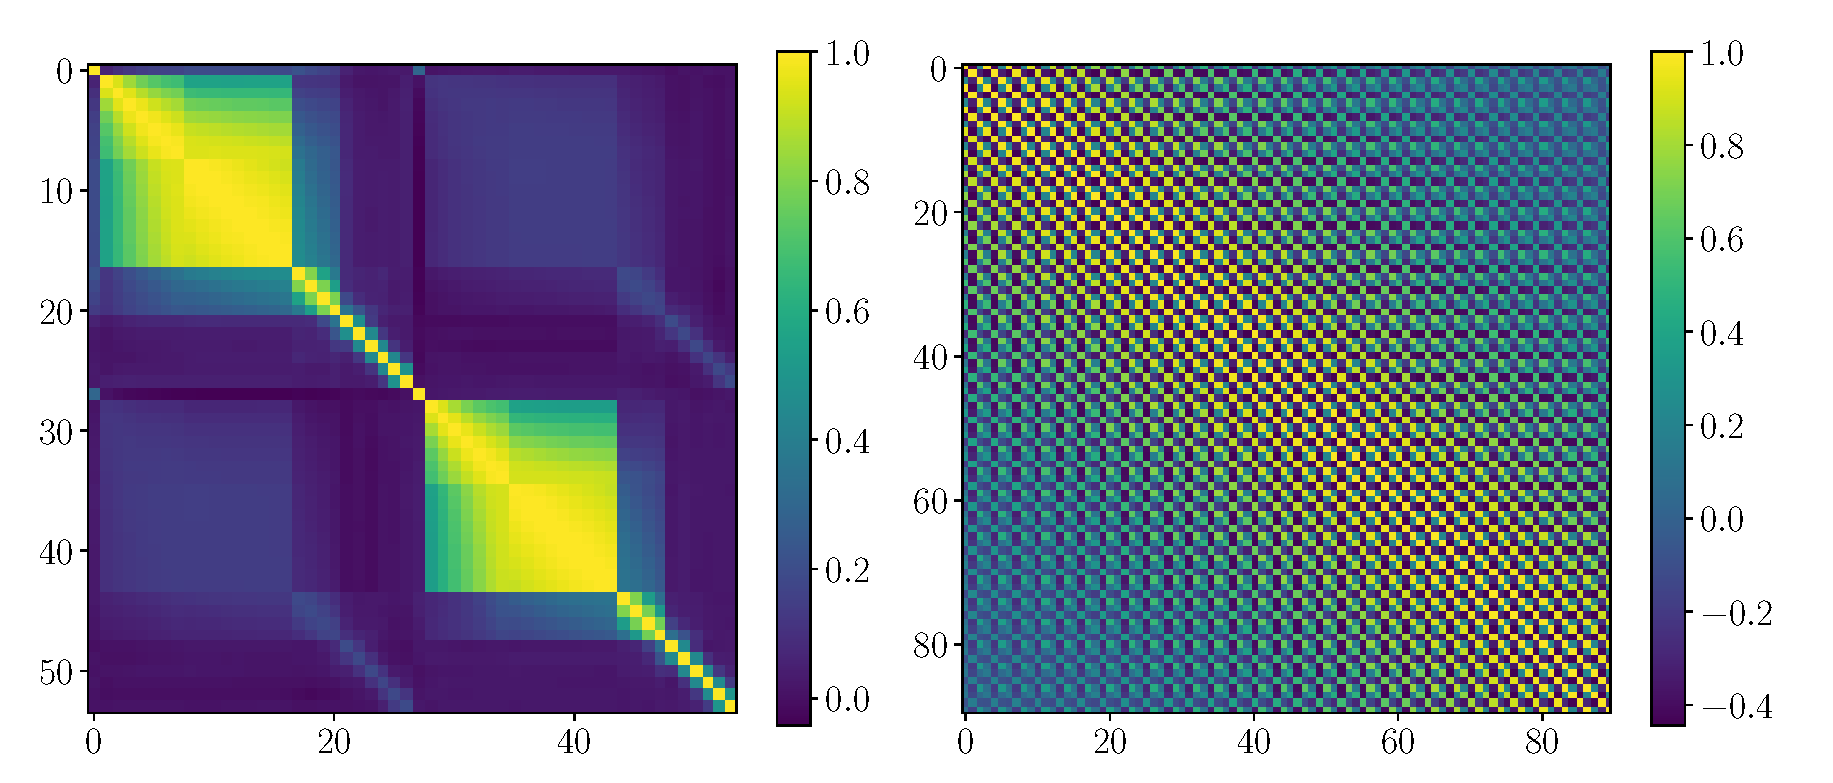
\includegraphics[width=\linewidth]{figs/corr_matrix.eps}
	\caption{Correlation matrices for $\bX$ and $\bY$}
	\label{fig:corr_matrix}
\end{figure}

We apply the QPFS algorithm with SymImp strategy for different values of~$\alpha_3$ coefficient according to formulas~\eqref{eq:alphas3}.
The dependence between target scores~$\bz_y$ with respect to~$\alpha_3$ for different values of~$k$ is shown in Figure~\ref{fig:features_vs_alpha_ecog}.
If we predict wrist coordinates only for one timestamp $k = 1$, targets scores are almost the same.
It tells about the independence between $x$, $y$, and $z$ coordinates.
For $k = 2$ and $k = 3$ the scores of some targets become zero when~$\alpha_3$ increases.
The vertical lines correspond to the optimal value of coefficient~$\alpha_3$ obtained by~\eqref{eq:alpha_3}. 
The importances~$\ba_y$ for this value of~$\alpha_3$ are similar. 
It means that the algorithm does not distinguish the targets for $k=1, 2, 3$.

\begin{figure}[h]
	\begin{minipage}{.5\linewidth}
		\subfloat[k=1]{\label{fig:autoreg_step1}
			\includegraphics[width=\linewidth]{figs/features_vs_alpha_ecog_3.pdf}}
	\end{minipage}%
	\begin{minipage}{.5\linewidth}
		\subfloat[k=2]{\label{fig:autoreg_step2}
			\includegraphics[width=\linewidth]{figs/features_vs_alpha_ecog_6.pdf}}
	\end{minipage}\par\medskip
	\subfloat[k=3]{\label{fig:autoreg_step3}
		\includegraphics[width=\linewidth]{figs/features_vs_alpha_ecog_9.pdf}}

	\caption{Target importances~$\bz_y$ with respect to~$\alpha_3$ for QPFS with Symmetric Importance}
	\label{fig:features_vs_alpha_ecog}
\end{figure}

\hrulefill

We compare the proposed strategies of multivariate QPFS that are given in Table~\ref{tbl:summary} for the ECoG dataset. 
Firstly, we apply all methods to get feature importances. 
Then we fit linear model with increasing number of features. 
For each method the features are sorted by the obtained importances. 
We show how the described metrics are changed with the increasing feature set size. 
Figure~\ref{fig:ecog_3_1_metrics} illustrates the results for $k = 1$. 
Here all metrics values for RelAgg, SymImp, and MaxRel are quite similar. 
However, MaxMin and MinMax algorithms show worse performance. 
This behavious is possibly due to unreasonable penalty on the matrix~$\bY$.

The situation changes for predicting several timestamps. 
In this case the correlation in~$\bY$ matrix is crucial. 
Figure~\ref{fig:ecog_3_15_metrics} shows algorithms performance for $k = 15$. 
The test error is minimal for SymImp, MinMax, and MaxRel strategies.  
The RelAgg strategy shows almost the worst error rate.

\begin{figure}[h]
	\includegraphics[width=\linewidth]{figs/ecog_3_30_metrics.pdf}
	\caption{Metrics values for ECoG data with k = 30}
	\label{fig:ecog_3_15_metrics}
\end{figure}
\begin{table}[]
	\caption{}
	\centering
	\begin{tabular}{l|ccccc}
		\hline
		& RMSE  & $\|\ba\|_0$ & Spearman $\rho$ & $\ell_2$ dist \\ \hline
		RelAgg & 41.9 $\pm$ 0.1 & 27.0 $\pm$ 2.4 & 0.941 $\pm$ 0.005 & 0.14 $\pm$ 0.02   \\
		SymImp & 41.1 $\pm$ 0.1 & 198.6 $\pm$ 3.8 & 0.942 $\pm$ 0.008 & 0.03 $\pm$ 0.00   \\
		MinMax & 41.4 $\pm$ 0.2 & 92.4 $\pm$ 8.2 & 0.933 $\pm$ 0.007 & 0.10 $\pm$ 0.01   \\
		MaxMin & 41.7 $\pm$ 0.1 & 97.0 $\pm$ 4.4 & 0.950 $\pm$ 0.004 & 0.07 $\pm$ 0.01   \\
		MaxRel & 41.7 $\pm$ 0.0 & 37.6 $\pm$ 1.6 & 0.893 $\pm$ 0.012 & 0.17 $\pm$ 0.02  \\ \hline
	\end{tabular}
	\label{tbl:stability}
\end{table}

\begin{figure}
	\centering
	\includegraphics[width=\linewidth]{figs/ecog_prediction}
	\caption{}
	\label{fig:ecog_prediction}
\end{figure}

\newpage
\section{Conclusion}
The study investigates the problem of signal decoding in relation to modelling Brain Computer Interface. 
To build a stable edequate model, it was proposed to reduce dimensionality of the problem using the dependencies in both input and target spaces.
The partial least squares algorithm is considered as linear model for dimensionality reduction.
The quadratic programming approach is investigated as feature selection algorithm.
The multivariate extensions for the QPFS algorithms are proposed.
The algorithms solve feature selection in a single quadratic programming optimization problem.
The resulting feature subset includes non-correlated features which are relevant to the most difficult targets.

The computational experiments were carried out on the ECoG data. 
The resulting model predicts the limb position of an exoskeleton by brain signals.
The proposed algorithms outperforms the baseline algorithm and reduce the problem dimension significantly.

\bibliographystyle{unsrt}
\newpage
\bibliography{papers_thesis}

\end{document}
